% 9 variables in here:
% h_1 = 10.0, h_2 = 16.0, h_3 = 4.0, ux_1 = 0.0, ux_2 = 0.0, ux_3 = 0.0, uy_1 = 0.0, uy_2 = 0.0, uy_3 = 0.0
\begin{figure}[ht]
\centering
  \quad \subfloat[$SE_x^1$, $SE_y^3$] {
    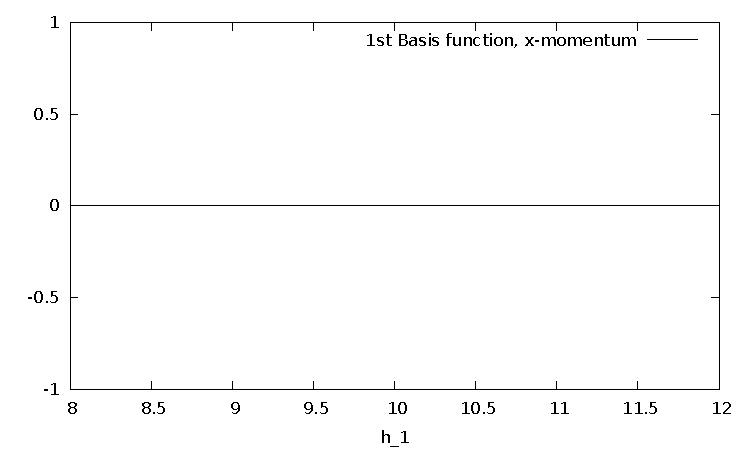
\includegraphics[scale=\zoomfactor]{{{ord1_differing_h2_h3_164/y_16.0_4.0_0.0_0.0_0.0_0.0_0.0_0.0f00}}}
  }
  \quad \subfloat[Remaining error terms, $SE_x^2$, $SE_x^3$, $SE_y^1$, $SE_y^2$] {
    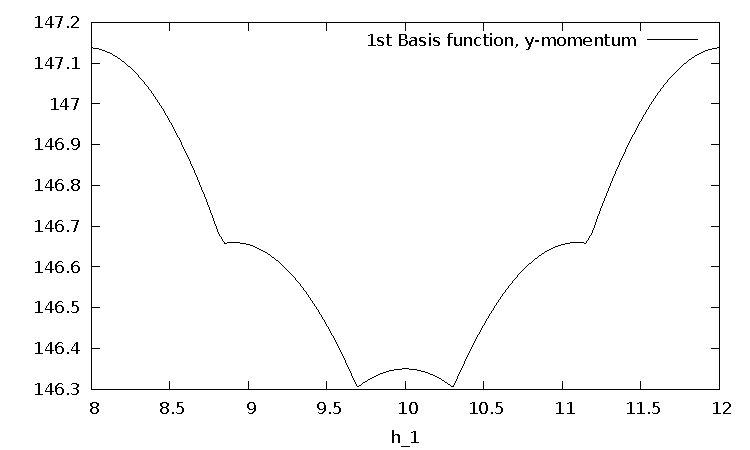
\includegraphics[scale=\zoomfactor]{{{ord1_differing_h2_h3_164/y_16.0_4.0_0.0_0.0_0.0_0.0_0.0_0.0f01}}}
  }
  % \quad \subfloat[] {
  %   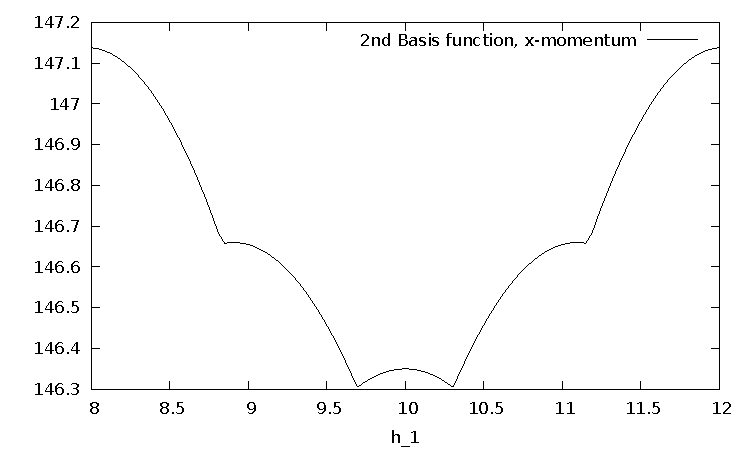
\includegraphics[scale=\zoomfactor]{{{ord1_differing_h2_h3_164/y_16.0_4.0_0.0_0.0_0.0_0.0_0.0_0.0f02}}}
  % }
  % \quad \subfloat[] {
  %   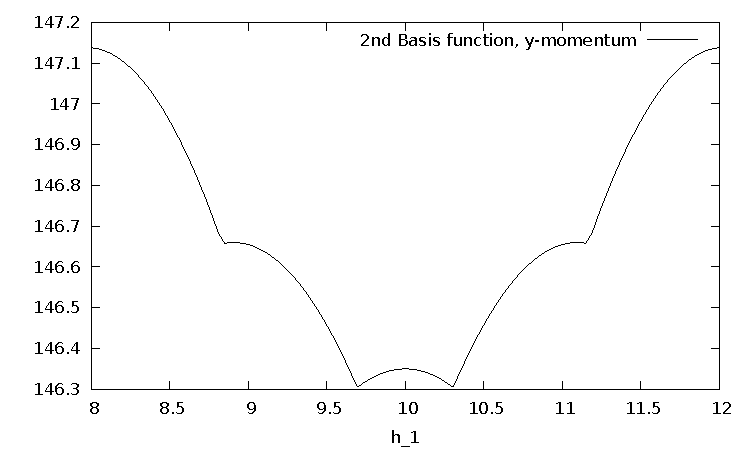
\includegraphics[scale=\zoomfactor]{{{ord1_differing_h2_h3_164/y_16.0_4.0_0.0_0.0_0.0_0.0_0.0_0.0f03}}}
  % }
  % \quad \subfloat[] {
  %   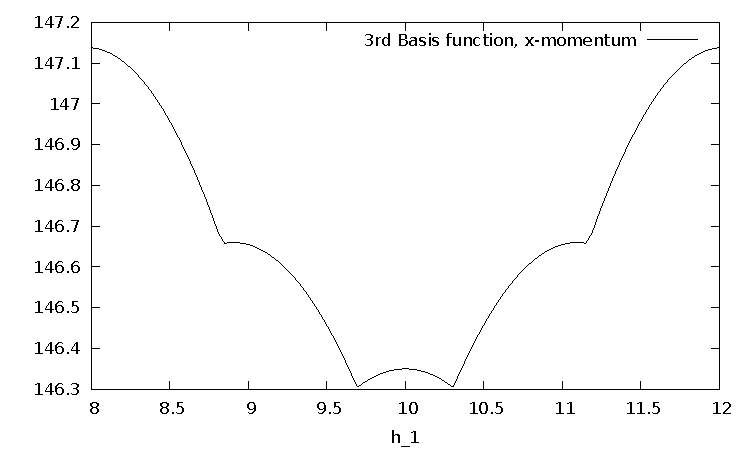
\includegraphics[scale=\zoomfactor]{{{ord1_differing_h2_h3_164/y_16.0_4.0_0.0_0.0_0.0_0.0_0.0_0.0f04}}}
  % }
  % \quad \subfloat[] {
  %   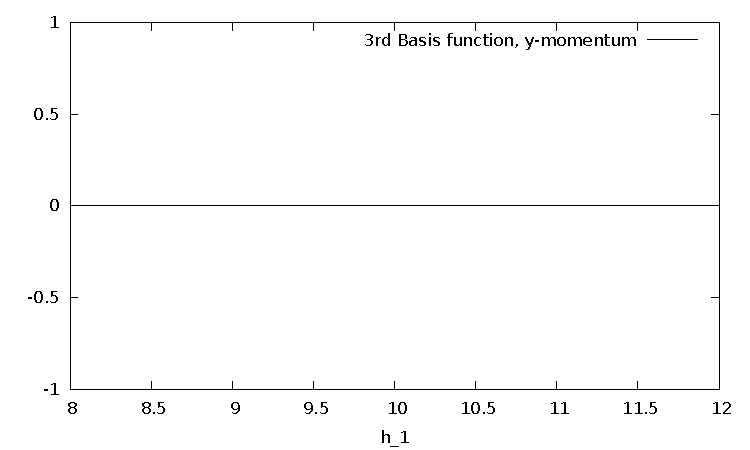
\includegraphics[scale=\zoomfactor]{{{ord1_differing_h2_h3_164/y_16.0_4.0_0.0_0.0_0.0_0.0_0.0_0.0f05}}}
  % }
\caption{All momentums are set to $0$, $h_2=16$ and $h_3=4$.}
\label{fig:ord1_differing_h2_h3_164}
\end{figure}

%%% Local Variables:
%%% TeX-master: "../results.tex"
%%% End:
